\documentclass{article}

\renewcommand{\familydefault}{\sfdefault}  %serifenlose Schrift
\usepackage{helvet} % Schrift: Helvetica


\usepackage{graphicx,graphics,tikz}
\usepackage{amsmath}
\usepackage{amsthm}
\usepackage{amsfonts}
\usepackage{amssymb}
\usepackage{marvosym} % to be able to show male and female symbols with: \Female and \Male
\usepackage{gensymb}
\usepackage[graphics,tightpage,active]{preview}
\PreviewEnvironment{tikzpicture}
\newlength\imagewidth
\newlength\imagescale

\begin{document}

\pgfmathsetlength{\imagewidth}{10cm} % desired displayed width of image
\pgfmathsetlength{\imagescale}{\imagewidth/2000} % pixel width of image
% adjust scale of tikzpicture (and direction of y) such that pixel
% coordinates can be used for drawing overlays:
\usetikzlibrary{backgrounds}

\begin{tikzpicture}[x=\imagescale,y=-\imagescale]

  % Insert Background Image place image (integer coordinates refer to

\node [text centered] at (0cm,1cm) {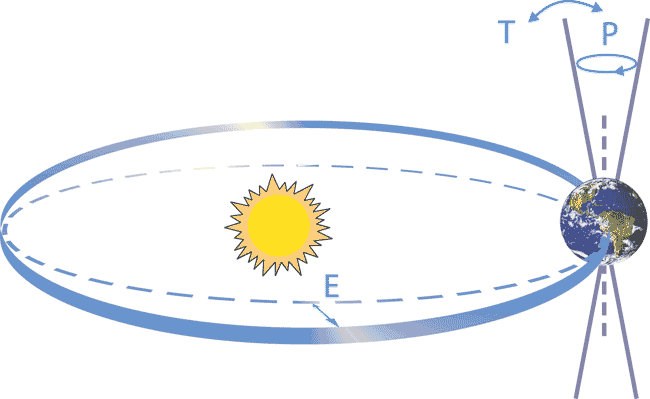
\includegraphics[width=2.5cm]{milankovich.png}};
\node [text centered,text width=3cm] at (0cm,1.8cm) {Milankovich cycles\\\vspace{-0.1cm}\tiny{IPCC2007}};

\node [text centered] at (-4cm,-0.2cm) {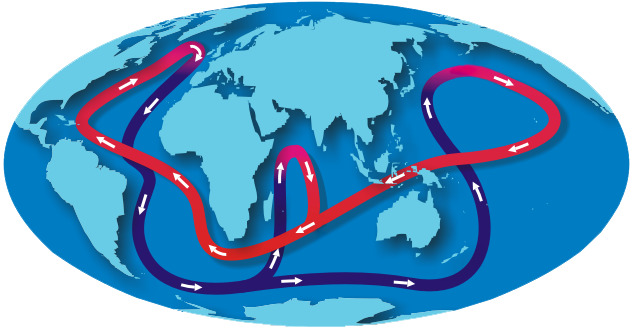
\includegraphics[width=1.5cm]{ConveyorBelt_NOAA.jpg}};
\node [text centered,text width=4cm] at (-4cm,-1.1cm) {\small{Ocean currents}\\\vspace{-0.1cm}\tiny{NOAA}};

\node [text centered,text width=2.5cm] at (0cm,-0.2cm) {\small{$CO_2$ fluctuations}};

\node [text centered] at (4cm,-0.2cm) {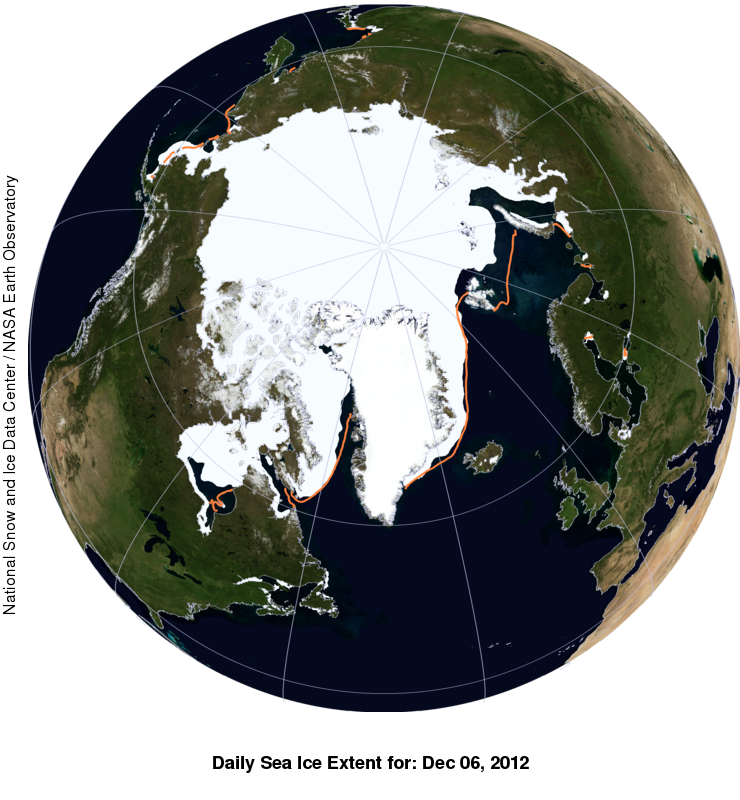
\includegraphics[width=1cm]{SeaIce_NASA.png}};
\node [text centered,text width=4cm] at (4cm,-1.1cm) {\small{Ice cover}\\\vspace{-0.1cm}\tiny{NASA}};




\draw [line width=0.03cm,-latex] (1.5cm,0.5cm) -- (3cm,0cm);
\draw [line width=0.03cm,-latex] (-1.5cm,0.5cm) -- (-3cm,0cm);
\draw [line width=0.03cm,-latex] (0cm,0.4cm) -- (0cm,0cm);



\draw [line width=0.03cm,-latex] (3cm,-.2cm) -- (0.8cm,-.7cm);
\draw [line width=0.03cm,-latex] (-3cm,-.2cm) -- (-0.8cm,-.7cm);
\draw [line width=0.03cm,-latex] (0cm,-0.3cm) -- (0cm,-.7cm);
%\draw [line width=0.03cm,-latex] (0cm,-2.5cm) -- (0cm,-2.9cm);


\node [text centered,text width=4cm] at (0cm,-2.1cm) {\textbf{Climate fluctuations}\\\vspace{-0.2cm}\tiny{NASA}};
\node at (0cm,-1.2cm) {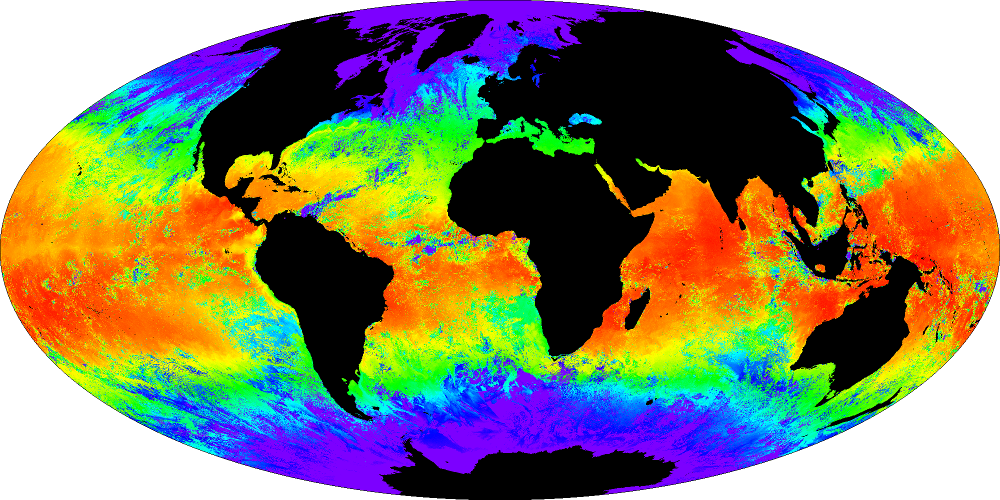
\includegraphics[width=2cm]{Nasa_global_SST.png}};


% \node at (0cm,-3.9cm) {\includegraphics[width=3cm]{Garrison-2010-Fig16_3.png}};
% \node [text centered,text width=4cm] at (0cm,-5.3cm) {\textbf{Species distribution}\\\vspace{-0.1cm}\tiny{\cite{Garrison2010}}};
\end{tikzpicture}

\end{document}